\documentclass{standalone}

\usepackage{tikzducks}


\begin{document}

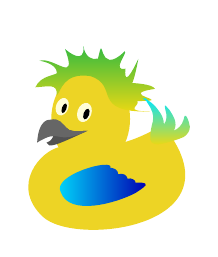
\begin{tikzpicture}
\duck[parrot,bill=gray!80!black]
\shade[left color=cyan!90!blue,right color=blue!70!black] \duckpathwing;
\shade[bottom color=yellow!70!brown, top color=green!40!teal] \duckpathcrazyhair;
\shade[bottom color=yellow!70!brown, top color=cyan!90!blue]
	 	(1.56,1.76) .. controls (1.60,1.74) and (1.62,1.72) .. (1.63,1.69) .. controls (1.67,1.63) and (1.71,1.55) .. (1.69,1.47) .. controls (1.67,1.40) and (1.65,1.31) .. (1.66,1.23) .. controls (1.66,1.20) and (1.69,1.19) .. (1.72,1.18) .. controls (1.77,1.17) and (1.82,1.19) .. (1.87,1.20) .. controls (1.94,1.22) and (2.01,1.24) .. (2.08,1.27) .. controls (2.13,1.30) and (2.16,1.35) .. (2.16,1.40) .. controls (2.15,1.45) and (2.14,1.50) .. (2.11,1.54) .. controls (2.08,1.55) and (2.09,1.50) .. (2.08,1.49) .. controls (2.06,1.42) and (2.01,1.37) .. (1.95,1.35) .. controls (1.93,1.33) and (1.97,1.36) .. (1.97,1.38) .. controls (1.99,1.44) and (1.97,1.50) .. (1.94,1.55) .. controls (1.91,1.60) and (1.89,1.64) .. (1.85,1.67) .. controls (1.83,1.68) and (1.85,1.63) .. (1.85,1.61) .. controls (1.87,1.55) and (1.87,1.48) .. (1.83,1.43) .. controls (1.83,1.50) and (1.80,1.56) .. (1.76,1.61) .. controls (1.72,1.67) and (1.67,1.71) .. (1.61,1.75) .. controls (1.61,1.76) and (1.60,1.76) .. (1.60,1.76) -- cycle;
\end{tikzpicture}

\end{document}
